\subsection{Data}
\subsubsection{Simulated dataset}
\label{sssection:simulateddata}
In order to assess calibration and power of LiMMBo, genotypes and phenotypes were simulated similar to strategies described in \citep{Loh2014,Casale2015}.  
\paragraph{Genotypes.} The synthetic genotypes were generated based on real genotype data from the European ancestry populations of the 1000 Genomes (1KG) Project (populations: CEU, FIN, GBR, IBS, TSI) \citep{Abecasis2012}. Depending on the cohort structure, each newly synthesised individual is assigned to \(N\) ancestors from the original 1KG Project and  their genome split into blocks of 1,000 SNPs (thereby retaining realistic LD structure between SNPs). For each SNP block, an ancestor is chosen at random and its genotype is copied to the individuals genome. Low numbers of \(N\) introduce relatedness among indivduals, whereas high numbers of \(N\) lead to low levels of structure and relatedness. By allowing random selection of the ancestors from the five subpopulations, population structure will be low, whereas predefining subpopulation of the ancestor can give rise to structured populations. Three distinct cohorts of 1,000 individuals each were generated: i) unrelated individuals, with population structure (unrelatedPopStructure): \(N=10\), prior assigment to ancestorial population , ii) unrelated individuals, no population structure (unrelatedNoPopStructure): \(N=10\), no prior assigment to ancestorial population and iii) related individuals, no population structure (relatedNoPopStructure): \(N=2\), no prior assigment to ancestorial population.  
\paragraph{Phenotypes.} For the power analyses, phenotypes were generated as the sum 
of three components: i) fixed genetic effects, ii) background genetic effects (based on population structure) and iii) and background noise effects. To assess calibration, only background genetic and noise effects contributed to the phenotypes. Each component had a percentage \(\theta\) of common effect, i.e. the effect was shared across traits and \((1- \theta)\)  independent effect. For each of the genotype cohorts described above, different phenotype scenarios depending on percentage of variance explained by genetics \(v_g\) (fixed and background genetic effects) and number of traits \(P\) were simulated: i) \(v_g={0.2, 0.5, 0.8}\) and ii) \(P={10, 20, ..., 100}\).


\subsection{Covariance estimation}
The LIMIX framework enables multi-trait LMM analyses for more than two traits and provides methods to decompose phenotypic variance \citep{Lippert2014}. In single-variant LMMs, typically two phenotypic variance components are assumed: i) a genetic component \(g\) and ii) a noise component \(\psi\) (Equations \ref{eq:lmm-uv} and \ref{eq:lmm-mv}). 
\noindent To estimate the variance decomposition (VD) into \(g\) and \(\psi\), the phenotype is described as the null model of the LMM:
\begin{equation}
\mathbf{y} = \mathbf{g}+\boldsymbol{\psi},\text{ }
\mathbf{g}\sim
\mathcal{N}\left(0,
\mathbf{C_g} \otimes \mathbf{R}\right),\text{ }
 \mathbf{\psi}\sim
\mathcal{N}\left(0,\mathbf{C_n} \otimes \mathbf{I_n}\right)
\label{eq:vd}
\end{equation}

The sample-by-sample covariances of the genetic and noise term, \(R\) and \(I_N\), are provided and the model estimates the trait-by-trait covariance matrices \(C_g\) and \(C_n\). The complexity of the VD is \(O(N^2 + t(NP^2 + NP^4))\) with \(N\) the number of samples, \(P\) the number of traits, and \(t\) the number of iterations of Broyden's method for optimising the restricted marginal likelihood (RML) of the parameter estimates. From this equation, it becomes evident that as the number of traits increases, the complexity increases by a power of four and explains why the LMM is not feasable for large trait sets. In order to to allow for multi-trait mapping of large trait sets, a bootstrapping-based approach was investigated. Instead of modeling all traits at the same time, a subset of \(p\) traits is randomly selected, the VD computed  and the $p \times p$ covariance matrices $C^*_g$ and $C^*_n$ recorded. This random selection with replacement is repeated \(n\) times such that each two traits are drawn together at least ten times, with \(n\) depending on the overall trait size \(P\) and the sampling size \(p\).  The challenge after the VD is to combine the bootstrap results in a way, that the resulting $C_g$ and $C_n$ are true covariance matrices, i.e. positive semi-definite matrices. Simply averaging values over all bootstrapping results leads to matrices with negative eigenvalues which have to be regularized to achieve positive semi-definiteness. The regularization leads to an overestimation of the trait variances (diagonal) compared to the trait-trait covariances (off-diagonal). In order to circumvent this overestimation, the unregularized averaged $C_g$ and $C_n$ are used as an initial guess to fit a residual sum of squares model over all bootstrap runs. The model makes use of cholesky decomposition of the matrix to be fitted, resulting in $\frac{1}{2}P(P+1)$ model parameters to be fitted. The fitting is achieved by using the BFGS optimizer, a limited memory quasi-Newton algorithm for solving large nonlinear optimization problems \citep{Byrd1995}.  $C_g$ and $C_n$ are fitted separately. The complexity of LiMMBo is \(O(N^2 + t_1(Np^2 + Np^4) + t_2(\frac{1}{2}P(P+1))\), which is the sum of the complexity of the VD as described above for the subset of \(p\) traits and the complexity of fitting the BFGS algorithm \(t_2\) times for the full trait set size \(P\). 


 
 \subsection{LiMMbo yields covariance estimates comparable to RML estimates}
For trait set sizes of up to 30 traits, the RML estimates of  $C_g$ and $C_n$ are possible. In order to compare the estimates derived from pure RML and from the combination of RML estimates of \(p\)-sized subset matrices (LiMMBo), the VD of the simulated phenotypes with \(P=(10,20,30)\) was estimated both via RML and LiMMBo for all phenotype setups (Section \ref{sssection:simulateddata}).  For \(P=10\), subsets of \(p=5\) were drawn, otherwise \(p=10\). $C_g$ and $C_n$ estimates of both methods were used in a any effect multi-variate LMM (Equation \ref{eq:lmm-mv}) across all genome-wide SNPs (mtGWAS). Statistical calibration of the mtGWAS was estimated by counting the number of tests that exceed a given threshold \(\alpha\) divided by the overall number of tests conducted (number of SNPs). Figure~\ref{fig:closedForm} shows the comparison of the false discovery rate (FDR) estimates of mtGWAS depending on the method of VD estimation, trait set size and genetic architecture. If the model is well calibrated, the FDR (depicted as bar charts in different transparency for both estimates) reaches as far or beyond the vertical line for the applied \(\alpha\) threshold. mtGWAS with LiMMBo-derived \(C_g\) and \(C_n\) estimates yields equally well calibrated results compared to the results from RLM estimates.

 \begin{figure}[hbtp]
	\centering
	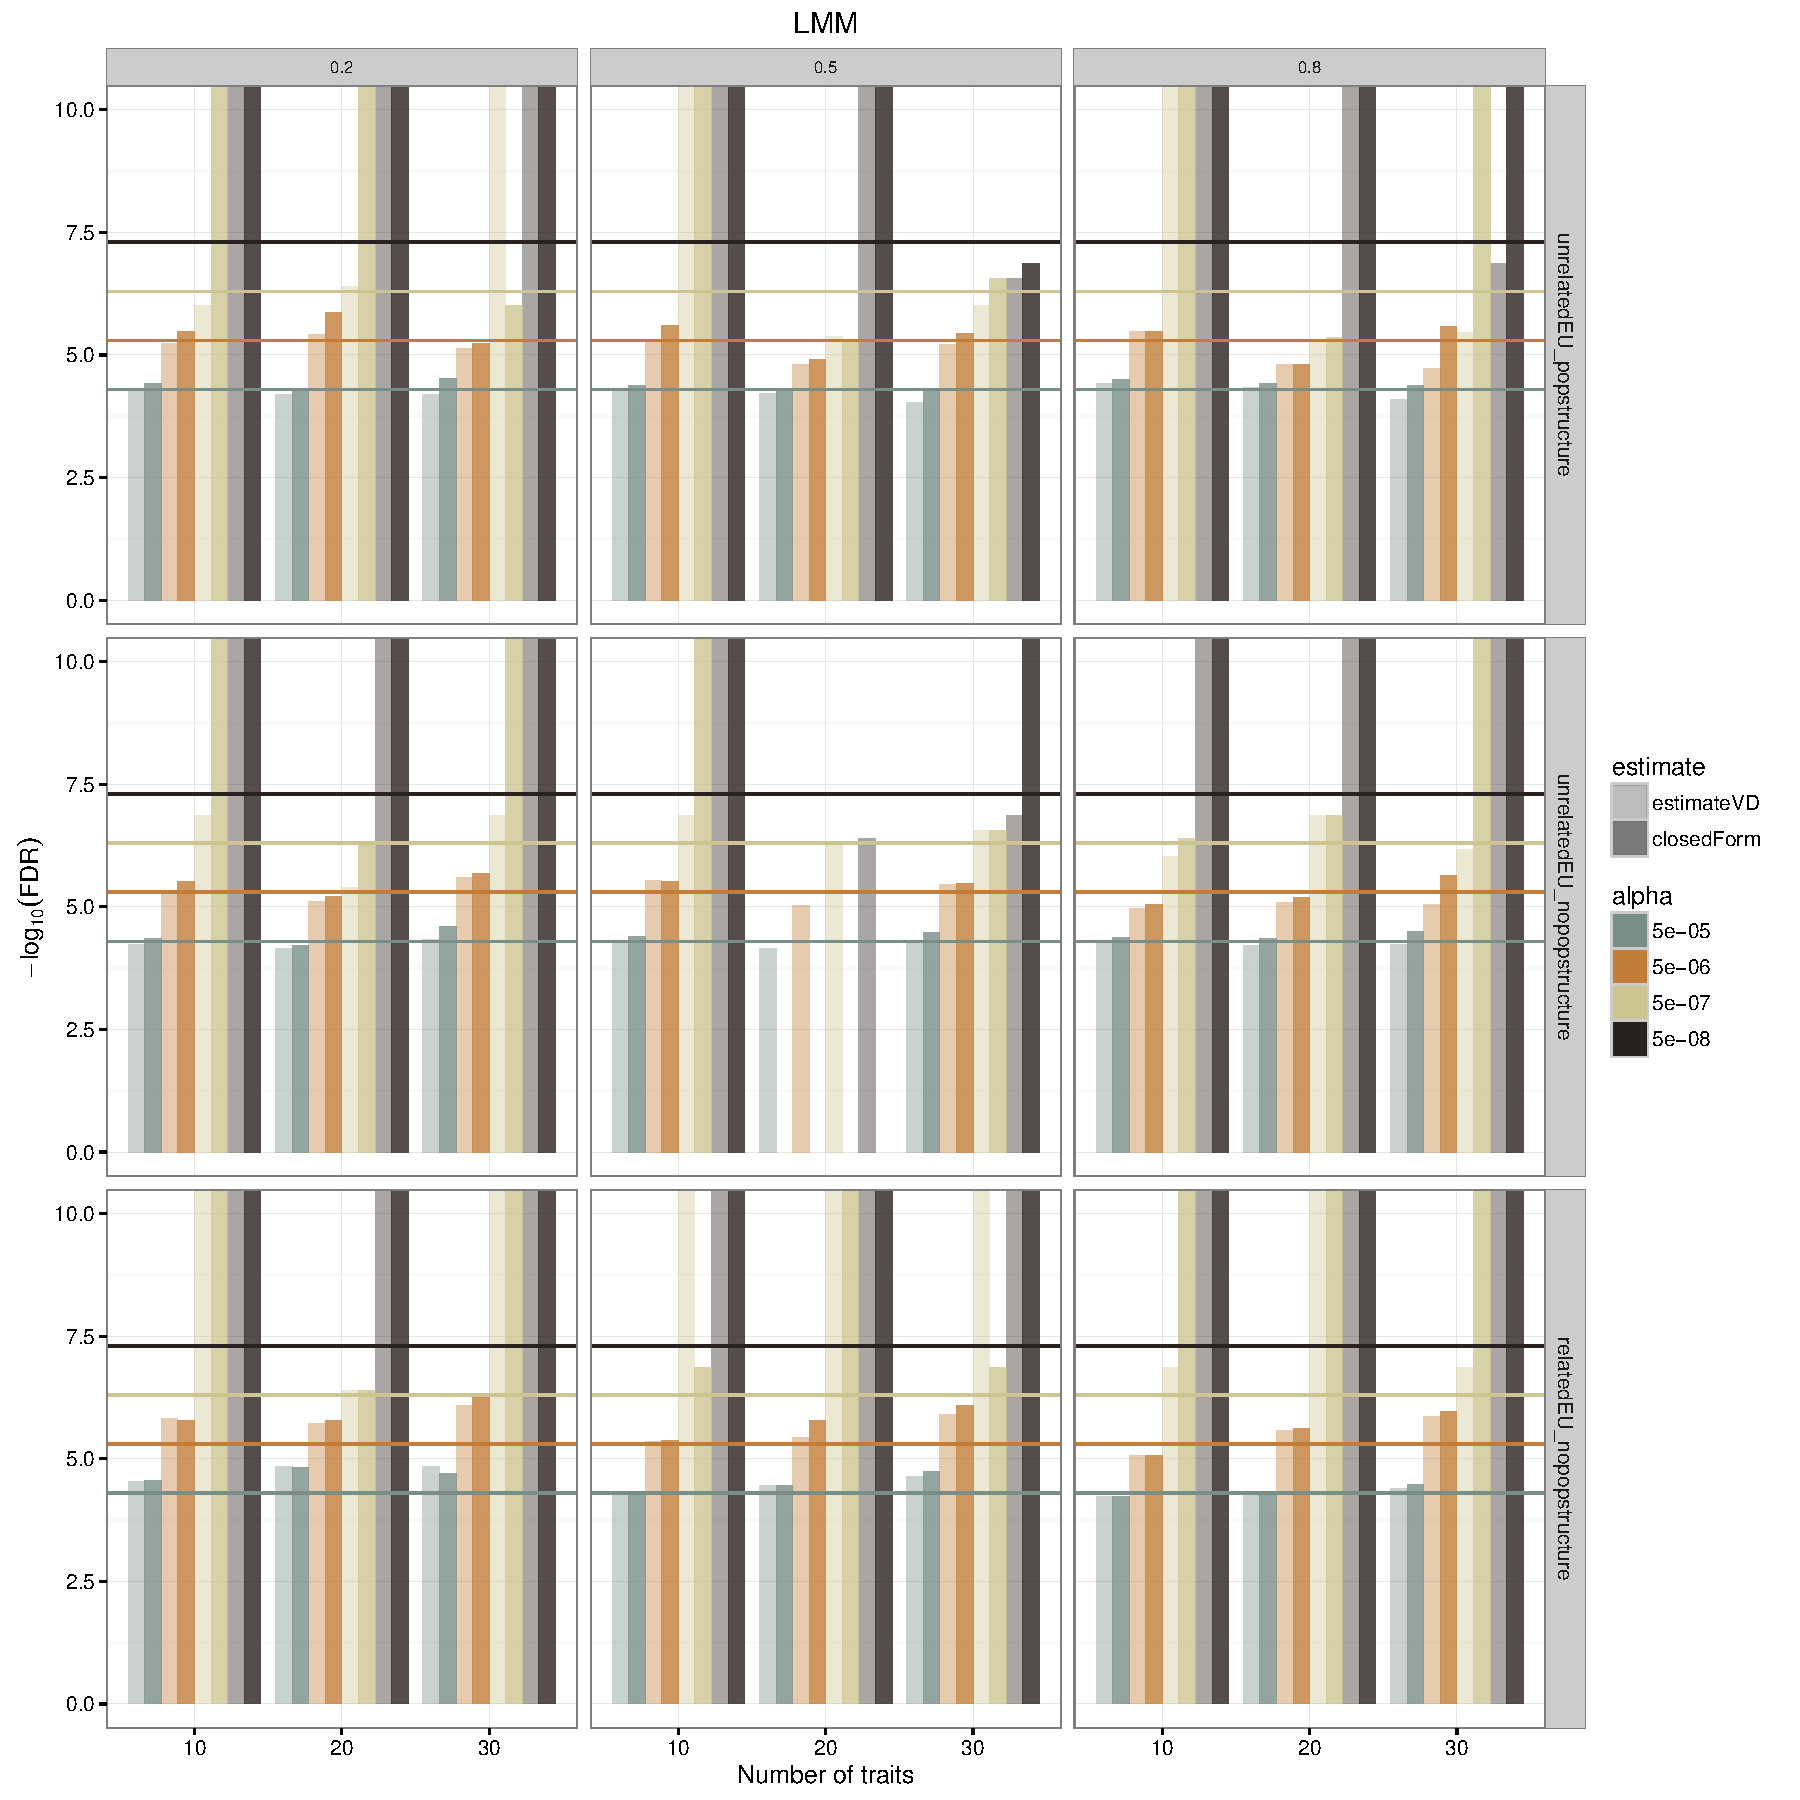
\includegraphics[trim = 0mm 0mm 0mm 0mm, clip, width=0.5\textwidth]{Chapter1/Figures/20161205_calibrationBGOnly_closedForm.pdf}
	\caption{\textbf{Comparison of LMM based on RLM trait-trait covariance estimates to LiMMBo-derived estimates.}  For each genetic architecture (unrelatedEU\_popstructure, unrelatedEU\_nopopstructure, relatedEU\_nopopstructure) and percentage of variance explained by genetics (0.2, 0.5, 0.8; purely by background genetic effects), three different trait set sizes (10, 20, 30) were simulated and the calibration of the model was assesed by mtGWAS with LiMMBo-derived (estimateVD) RLM estimates (closedForm) of \(C_g\) and \(C_n\). For calibrated models, the FDR (depicted as bar charts in different transparency for both estimates) reaches as far or beyond the vertical line for the applied \(\alpha\) threshold. Overall, estimates from both models yield equally well calibrated results.}
 	\label{fig:closedForm}
\end{figure}

 
 \subsection{Model choice for mtGWAS depends on relatedness and population structure}
 \label{ssection:modelchoice}
Figure~\ref{fig:modelchoice} shows the calibration of the mtGWAS for either the LM with the first ten principle components (LM-PC) of the kinship matrix as covariates \(F\) (Figure~\ref{fig:calibration-lmpc}; Equation~\ref{eq:lm-mv}) or the LMM  (Figure~\ref{fig:calibration-lmm}; Equation~\ref{eq:lmm-mv}). The model calibration strongly depends on the underlying genetic architecture of the cohort. In cohorts without relatedness and structure,  LM-PC is much better calibrated than the LMM, whereas the LMM outperforms the LM-PC in cohorts with related individuals.

\begin{figure}[!h]
	\centering
	\begin{subfigure}[b]{0.45\textwidth}
		%\hspace{3cm}
		\center
	\includegraphics[page=2, trim = 0mm 0mm 28mm 5mm, clip, scale=0.25]{Chapter1/Figures/20170105_calibrationBGOnly.pdf}
	\caption{\textbf{Linear model with PCs}}
 		\label{fig:calibration-lmpc}
	\end{subfigure}
	~
	\begin{subfigure}[b]{0.45\textwidth}
		%\hspace{3cm}
		\center
	\includegraphics[page=3, trim = 0mm 0mm 0mm 5mm, clip, scale=0.25]{Chapter1/Figures/20170105_calibrationBGOnly.pdf}\\
	\caption{\textbf{Linear mixed model}}
 		\label{fig:calibration-lmm}
	\end{subfigure}
	\caption{\textbf{Calibration of different models depending on population structure, number of traits and percentage of genetic variance.} (a) The LM set-up is reasonably well-calibrated for populations of unrelated individuals (upper two panels) across all trait sizes but is no calibrated for populations wtih high inter-individual relatedness especially in cases with a strong underlying genetic cause of the trait. (b) The LMM is well-calibrated up to trait set sizes of 30-40 traits for unrelated populations, but loses calibration for larger trait set sizes (upper two panels). It stays well calibrated across all trait sizes for populations with related individuals (lower panel).}
 	\label{fig:modelchoice}
\end{figure}

